%Bemerkung: Diese Datei wird über den \input{<name>.tex} in einer anderen .tex Datei %eingebunden. Daher müsst ihr euren Kram einfach nur noch runterschreiben
%Beispielsweise: 
\section{Software - Design}
\subsection{Usecases}
The flying software is definied by seven different usecases and three actors. \\ \\
The \textit{Controller actor} represents the most complex actor system in this project. It uses nine external ADC to measure the temperature or the resistance of the six strain gauges per signal processing unit (SPU). \\ \\ 
The usecase \textit{External ADC} describes the SPI communication to the nine external ADCs. One ADC is used for one channels at a sample rate of min. 800SPS up to 2kSPS. There will be four strain gauges conntected by a wheatstone bridge.\\ \\
The temperatur sensors will be connected by three of the  nine external ADCs. The sample rate will be at 10 to 20 SPS. \\ \\
\textit{Telemetry} covers each communication with the REXUS Serivce Module. Each communication will be initialized by the \textit{Controller}.\\ 
The \textit{Memory Usage} usecase describes how the memory is used. It is called each time the $\mu C$ saves something to flash memory. The controller have to save each measurment result and meta information about the flight, communication quality and in-flight problems. This usecase includes \textit{Write To Memory}, \textit{Reset Memory} and \textit{Read From Memory}. \\ \\
The \textit{DAPI} for \textit{D}ata \textit{a}nd \textit{p}rogramming  \textit{i}nterface usecase, describes the communication from ground station software to the microcontroller. \textit{DAPI} includes \textit{Memory Usage}.\\ \\
See Figure \ref{fig:usecase} as reference. 
\pagebreak
\begin{figure}[htb]
	\centering
	  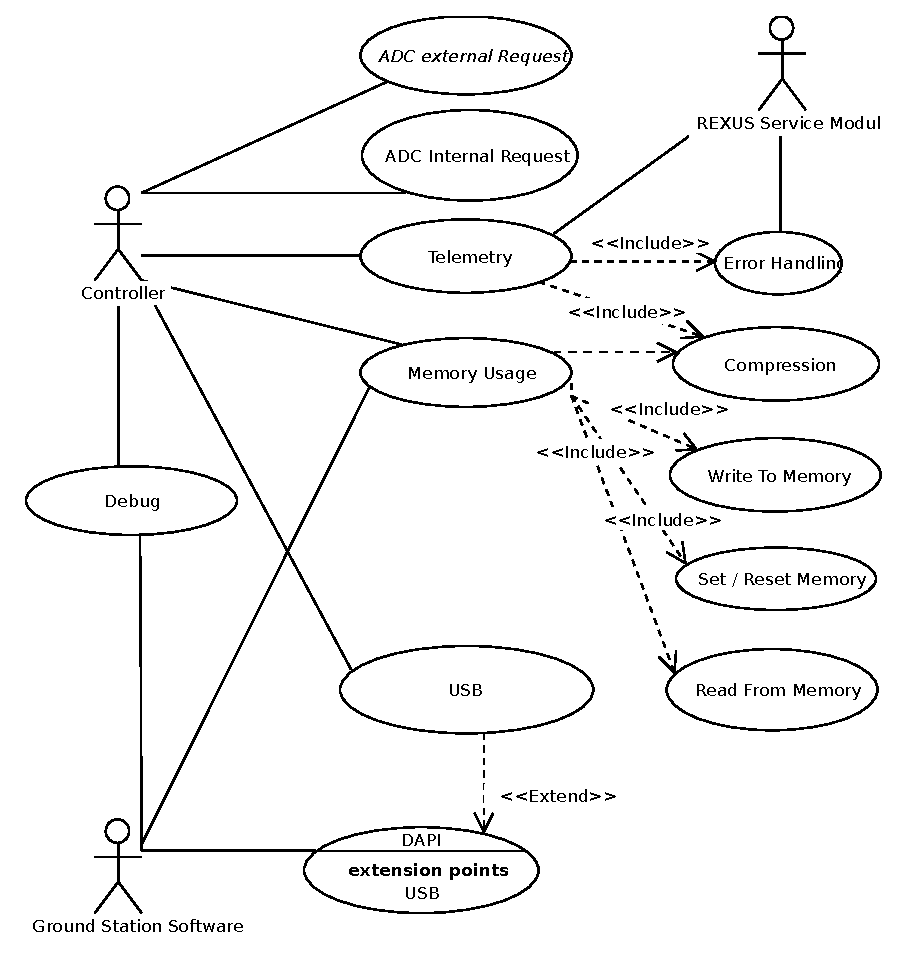
\includegraphics{SoftwareDesign/HERMESS_USECASE.eps}
	\caption{Usecases}
	\label{fig:usecase}
\end{figure}
\pagebreak
\begin{figure}[htb]
	\centering
	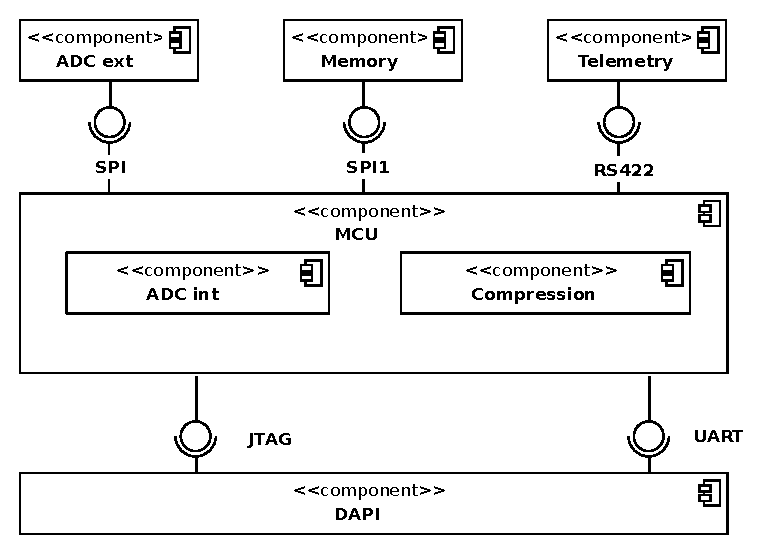
\includegraphics{SoftwareDesign/Components.eps}
	\caption{Component Diagramm}
\end{figure} \noindent
The components are \textit{ADC ext}, \textit{Memory}, \textit{Telemetry}, \textit{MCU}, \textit{Ground Station Software} and \textit{DAPI}. There four communication interfaces two of them are \textit{SPI}, one time \textit{RS422} and \textit{UART}.\\ \\
The component \textit{ADC ext} describes the communication with the external ADCs. This communication is SPI bases and works via chip select. The six strain gauge ADCs will be connected to one SPI. Another SPI will be used for the temeperature measurment. \\ \\
The \textit{Memory} component  describes two 128 Mbyte flash memory blocks each of then  is conntect to its own SPI. \\ \\
The \textit{Telemetry} component is the onboard REXUS Service Module, the communication will be maintained by a RS422 interface. \\ 
Component \textit{MCU} descibes the main controller, all components execpt the external ADC, Telementry, DAPI and Memory are not implmeneted on this MCU. The MCU provides and describes the interfaces used for communication. \\ \\
The \textit{DAPI} component is conntect to the \textit{MCU} by two diffrent interfaces. Second it is communicating with the \textit{MCU} via UART at a BAUD rate about 115200, 8, n 1 for memory usage and system maintance. 